\begin{figure}[H]
	\centering
	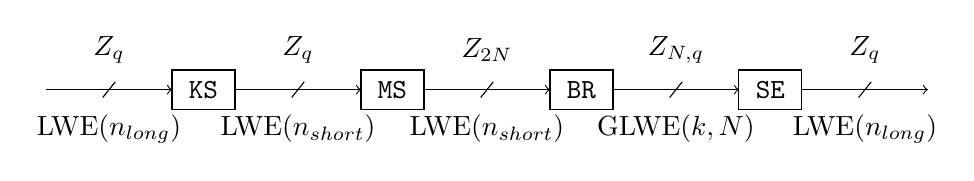
\begin{tikzpicture}[xscale=0.8,yscale=0.5]
		\draw[] (2, 0) rectangle (3, 1) node[pos=0.5,color=black]{$\texttt{KS}$} ;
		\draw[] (5, 0) rectangle (6, 1) node[pos=0.5,color=black]{$\texttt{MS}$} ;
		\draw[] (8, 0) rectangle (9, 1) node[pos=0.5,color=black]{$\texttt{BR}$} ;
		\draw[] (11, 0) rectangle (12, 1) node[pos=0.5,color=black]{$\texttt{SE}$} ;
		
		\draw[->] (0, 0.5) -- (2, 0.5);
		\draw[->] (3, 0.5) -- (5, 0.5);
		\draw[->] (6, 0.5) -- (8, 0.5);		
		\draw[->] (9, 0.5) -- (11, 0.5);
		\draw[->] (12, 0.5) -- (14, 0.5);
		
		\draw (0.9, 0.3) -- (1.1, 0.7);
		\draw (1.0, -0.5) node{LWE$(n_{\text{long}})$} ;
		\draw (1.0, 1.5) node{$\mathbb{Z}_q$} ;
		\draw (3.9, 0.3) -- (4.1, 0.7);
		\draw (4.0, -0.5) node{LWE$(n_{\text{short}})$} ;
		\draw (4.0, 1.5) node{$\mathbb{Z}_{q}$} ;
		\draw (6.9, 0.3) -- (7.1, 0.7);
		\draw (7.0, -0.5) node{LWE$(n_{\text{short}})$} ;
		\draw (7.0, 1.5) node{$\mathbb{Z}_{2N}$} ;
		\draw (9.9, 0.3) -- (10.1, 0.7);
		\draw (10.0, -0.5) node{GLWE$(k, N)$} ;
		\draw (10.0, 1.5) node{$\mathbb{Z}_{N, q}$} ;
		\draw (12.9, 0.3) -- (13.1, 0.7);
		\draw (13.0, -0.5) node{LWE$(n_{\text{long}})$} ;
		\draw (13.0, 1.5) node{$\mathbb{Z}_q$} ;	
	\end{tikzpicture}
	\caption{\label{fig:inside_pbs} Types and shapes of ciphertexts inside a PBS.}
\end{figure}